\documentclass[11pt]{article}

\usepackage[utf8]{inputenc}
\usepackage[margin=1in]{geometry}
\usepackage{hyperref}
\usepackage{graphicx}
\usepackage{booktabs}
\usepackage{amsmath}
\usepackage{amssymb}
\usepackage{xcolor}
\usepackage{natbib}
\usepackage{tikz}
\usetikzlibrary{arrows.meta, positioning, shapes.geometric}

\hypersetup{
  colorlinks=true,
  linkcolor=blue,
  citecolor=blue,
  urlcolor=blue
}

\title{Bi-Temporal Incident Memory on a Property Graph:
Hand-Rolled Graphiti-on-FalkorDB with No-LLM-at-Retrieval
Hybrid Recall and Reflexion Lessons}

\author{Victor Robin\\ BlueRobin (independent homelab research)}

\date{June 2026}

\begin{document}

\maketitle

\begin{abstract}
Large-language-model (LLM) agents that perform root-cause analysis (RCA) on
production incidents are, by default, amnesiac: each invocation starts from a
blank context window, re-derives the same conclusions about recurring faults,
and cannot say ``this was the cause last March, but a config change has since
superseded it.'' This paper describes the learning subsystem of the BlueRobin
Debug Agent (\textbf{FEAT-027}, increment~6), a hand-rolled bi-temporal
incident-memory subgraph built on the \emph{existing} FalkorDB property graph
rather than a dedicated memory framework. We deliberately re-implement the
Graphiti / Zep pattern \citep{rasmussen2025zep} in .NET---not the Python
\texttt{graphiti-core} library, and not \texttt{mem0}---to fit a single 2~GiB
graph store and a hard $\approx$50~EUR/month budget. Each concluded incident
becomes a \texttt{MemoryEpisode} joined to deduplicated \texttt{MemoryEntity}
facts by \texttt{MENTIONS} / \texttt{RESOLVED\_BY} / \texttt{SUPERSEDES} edges
that carry \emph{both} valid-time (\texttt{t\_valid} / \texttt{t\_invalid}) and
ingestion-time (\texttt{ingested\_at}); supersession invalidates an interval but
never deletes, enabling as-of queries. Retrieval is a hybrid,
\textbf{no-LLM-at-retrieval} engine: three legs---semantic Qdrant kNN over
bge-m3 1024-d embeddings, BM25 lexical, and graph-BFS over the bi-temporal
subgraph---fused by Reciprocal Rank Fusion \citep{cormack2009rrf} with a
Generative-Agents \citep{park2023generative} recency $\times$ importance $\times$
relevance tie-break, with a structural sentinel proving no model is consulted on
the retrieval path. We add Reflexion-style post-incident lessons
\citep{shinn2023reflexion} and a Voyager-style skill store
\citep{wang2023voyager}, and a code$\leftrightarrow$graph embedding join via
\texttt{CodeUnit.embedding\_ref}. We are explicit that this is a
systems/experience report: the memory subsystem ships shadow-first, the internal
eval is a self-seeded 9-incident set, and the agent remains advisory and
human-in-the-loop by design.
\end{abstract}

\section{Introduction}

The first four papers in this series described how the BlueRobin Debug Agent
localizes a fault: a personalized-PageRank ``blame propagation'' pre-rank, a
five-term re-normalizing score blend with a parameter-free BARO change-point term
\citep{pham2024baro}, an externalized verification-gate finite-state machine that
forbids the model from grading its own homework, and an eval harness that gates
every merge. All of that machinery operates \emph{within a single incident}. It
throws away everything the moment the RCA loop concludes.

That is a real and well-documented failure mode. The MAST taxonomy of agentic
failures \citep{cemri2025mast}, built from 310 ITBench traces, lists
\textbf{memory loss} among the dominant categories alongside incorrect
self-verification and premature termination. An agent that cannot remember that
\texttt{authelia} has gone down twice before for the same OIDC reason will
re-investigate from scratch each time, burning tokens against a hard
20~EUR/month LLM ceiling and offering the on-call human nothing they did not
already know.

The naive fix---stuff prior incident text into the prompt---fails for three
reasons. First, \textbf{cost and latency}: full-context memory is the most
expensive possible design; the literature reports roughly 90\% token and roughly
91\% p95-latency reductions from structured retrieval over full-context replay
\citep{chhikara2025mem0}. Second, \textbf{staleness}: a flat log cannot represent
that a fact was true until a change invalidated it---exactly the bi-temporal
correction RCA needs. Third, and most subtly, \textbf{retrieval-time
hallucination}: if you ask an LLM to \emph{choose} which past incidents are
relevant, you have reintroduced the model into the one place it should not
be---the grounding path. Graphiti's central claim is that hybrid retrieval
(semantic + BM25 + graph traversal) requires \textbf{no LLM at retrieval} and
still achieves a P95 near 300~ms, near-constant in graph size
\citep{rasmussen2025zep}.

This paper's contributions are deliberately modest and engineering-shaped:

\begin{itemize}
  \item \textbf{A hand-rolled bi-temporal incident-memory subgraph} that reuses
    the platform's already-deployed FalkorDB instead of standing up a dedicated
    memory service, re-implementing the Graphiti bi-temporal pattern in .NET
    because the reference library is Python/TS and a sidecar breaks the budget.
  \item \textbf{A no-LLM-at-retrieval hybrid recall} with three fail-open legs
    fused by Reciprocal Rank Fusion (RRF, $k=60$), a Generative-Agents recency
    tie-break, and a structural sentinel (\texttt{\_llmRetrievalProbe}) that
    fails a unit test if any LLM is consulted at retrieval.
  \item \textbf{Supersession without deletion}---invalidate-an-interval semantics
    and an explicit as-of query---so the agent can answer ``what was the cause
    \emph{as of} time~$T$.''
  \item \textbf{Reflexion lessons and a Voyager-style skill store}, plus a
    \textbf{code$\leftrightarrow$graph embedding join} via
    \texttt{CodeUnit.embedding\_ref} so a recalled incident links back to the
    source it implicated.
  \item \textbf{A cost-and-honesty framing}: the whole stack runs in a
    $\approx$50~EUR/month homelab, ships shadow-first, and is evaluated against a
    self-seeded benchmark we openly call oversimplified.
\end{itemize}

\section{Related Work}

\paragraph{Temporal knowledge-graph agent memory.}
The direct ancestor is Zep / Graphiti \citep{rasmussen2025zep}, which introduces
bi-temporal edges---distinguishing the \emph{valid time} of a fact
(\texttt{t\_valid} / \texttt{t\_invalid}) from its \emph{ingestion time}---and a
hybrid retrieval combining semantic cosine, BM25, and breadth-first graph
traversal with \textbf{no LLM at retrieval}, reporting a P95 around 300~ms and
$+18.5\%$ on LongMemEval at roughly 90\% lower latency than full-context replay.
The open-source \texttt{graphiti-core} defaults to Neo4j and also supports
FalkorDB, but is implemented in Python/TypeScript. We adopt the \emph{pattern},
not the library (discussed in Section~\ref{sec:impl}).

\paragraph{Other memory architectures.}
Mem0 \citep{chhikara2025mem0} frames memory as an extract$\to$update pipeline
(ADD / UPDATE / DELETE / NOOP) and reports roughly 90\% token and roughly 91\%
p95-latency savings versus full context. MemGPT / Letta \citep{packer2023memgpt}
treats the LLM as an OS managing tiered virtual context through tool calls. A-MEM
\citep{xu2025amem} builds Zettelkasten-style atomic notes with dynamic linking
and memory evolution. We reject \texttt{mem0} and the \texttt{graphiti-core}
sidecar primarily on cost and operational grounds, not capability
(\textbf{ADR-042}).

\paragraph{Agent learning patterns.}
Reflexion \citep{shinn2023reflexion} converts an episode into a verbal
self-reflection stored in a buffer, improving downstream success (HumanEval
$80 \to 91\%$); we render an analogous post-incident ``lesson.'' Voyager
\citep{wang2023voyager} maintains an ever-growing skill library of executable
code, which maps cleanly to a durable runbook/skill store that mitigates
catastrophic forgetting. Generative Agents \citep{park2023generative} defines the
canonical memory-stream score---\textbf{recency $\times$ importance $\times$
relevance}---which we reuse as the fusion tie-break.

\paragraph{Retrieval fusion.}
Reciprocal Rank Fusion \citep{cormack2009rrf} combines ranked lists from
heterogeneous retrievers by summing $1/(k + \mathrm{rank})$; it is parameter-light
(one constant, conventionally $k=60$) and rewards items appearing across multiple
lists. This is exactly the property we want from three orthogonal recall legs.

\paragraph{RCA-specific memory reuse.}
RCACopilot \citep{chen2024rcacopilot} is the strongest ``this pattern deploys''
evidence: retrieval-augmented root-cause \emph{category} prediction, reported in
production for over four years across more than thirty teams, with accuracy up to
0.766. It validates the core thesis that retrieving similar past incidents
materially helps an LLM diagnose new ones. The broader survey consensus
\citep{survey2024rca} is that LLM-only RCA ``lacks structural grounding and risks
hallucinated suggestions,'' and that a graph supplies that grounding. Our base
investigation loop is a ReAct-style \citep{yao2022react} tool loop, and we draw on
template-triple-to-natural-language serialization \citep{wu2024simple} when a
retrieved subgraph is rendered for the model.

\section{Method / Architecture}

\subsection{Why a subgraph, not a database}

The incident memory is not a separate store. It is a labelled subgraph inside the
same \texttt{bluerobin\_stack} FalkorDB property graph (\textbf{ADR-021}) that
already holds the platform's topology, telemetry-derived dependency edges, change
history, and prior RCA outcomes. Memory writes therefore reuse the single-writer
discipline of \texttt{GraphIngestor}, the parameterised Cypher templates of
\texttt{StackGraphCypher} (\textbf{SEC-SG-4}), and the ADR-021 provenance bundle
(\texttt{source}, \texttt{status}, \texttt{confidence\_score}) carried on every
node and edge. This is the central engineering choice (\textbf{FEAT-027},
\textbf{FR-SG-46}, \textbf{ADR-042}~D1): the memory model is ``the .NET Graphiti
pattern on FalkorDB, hand-rolled.''

\subsection{The bi-temporal schema}

Two node labels and three edge types form the memory subgraph
(Table~\ref{tab:schema}).

\begin{table}[ht]
\centering
\caption{The bi-temporal incident-memory subgraph.}
\label{tab:schema}
\begin{tabular}{llp{5.2cm}}
\toprule
Element & Kind & Notable properties \\
\midrule
\texttt{MemoryEpisode} & node & natural key \texttt{incident\_fingerprint}; \texttt{summary\_nl}, \texttt{resolution\_nl}, \texttt{concluded\_at}, \texttt{ingested\_at}, \texttt{t\_valid} \\
\texttt{MemoryEntity}  & node & natural key \texttt{entity\_type|entity\_ref}; a deduplicated fact entity (service, datastore, change, etc.) \\
\texttt{MENTIONS}      & edge (episode$\to$entity) & \texttt{t\_valid}, \texttt{t\_invalid}, \texttt{ingested\_at}, provenance \\
\texttt{RESOLVED\_BY}  & edge (episode$\to$entity) & the resolving fact; same bi-temporal triple \\
\texttt{SUPERSEDES}    & edge (episode$\to$episode) & lineage when a later episode corrects an earlier fact \\
\bottomrule
\end{tabular}
\end{table}

The defining property is \textbf{two independent time axes} on each
\texttt{MENTIONS} / \texttt{RESOLVED\_BY} edge:

\begin{itemize}
  \item \textbf{Valid-time}---\texttt{t\_valid} / \texttt{t\_invalid}---\emph{when
    the fact was true in the world}. A \texttt{MENTIONS} edge with
    \texttt{t\_invalid IS NULL} is currently valid; setting \texttt{t\_invalid}
    closes the interval.
  \item \textbf{Ingestion-time}---\texttt{ingested\_at}---\emph{when the agent
    learned it}. This lets the system reason about what it knew at a given moment,
    independent of when the fact was actually true.
\end{itemize}

Supersession never deletes. When a later episode establishes that a previously
recorded cause no longer holds (for example, a config change replaced the
offending one), \texttt{SupersedeMemoryFactAsync} performs two parameterised
writes: it \textbf{invalidates} the prior interval (\texttt{InvalidateMemoryFact}
sets \texttt{t\_invalid}, never \texttt{DELETE}) and writes a \texttt{SUPERSEDES}
lineage edge from the new episode to the prior one. The audit trail is preserved
in full.

This in turn enables an \textbf{as-of query}. \texttt{RecallMemoryFactAsOf}
returns the entity that a given episode mentioned \emph{as of} time~$T$ using the
canonical bi-temporal predicate:

\begin{verbatim}
MATCH (e:MemoryEpisode {incident_fingerprint: $fp})
      -[m:MENTIONS]->(n:MemoryEntity)
WHERE n.entity_type = $type AND n.entity_ref = $ref
  AND m.t_valid <= $asOf
  AND (m.t_invalid IS NULL OR m.t_invalid > $asOf)
RETURN n.entity_ref
\end{verbatim}

Every memory template is a constant string with bound parameters
(\textbf{SEC-SG-4}); relationship types and labels---which Cypher forbids
parameterising---are selected only from fixed, code-supplied sets. Writes are
idempotent \texttt{MERGE}-on-natural-key. The whole surface is \textbf{fail-open}
(\textbf{NFR-SG-2}): an unreachable graph or a malformed reply yields \texttt{null}
or an empty list, never an exception, so the RCA loop continues on its tool floor
even if memory is down.

\subsection{Hybrid recall with no LLM at retrieval}
\label{sec:recall}

Recall is the heart of the subsystem (\textbf{FR-SG-47}, \textbf{NFR-SG-16},
\textbf{ADR-042}~D4). \texttt{RelatedIncidentRecall.Recall} runs three orthogonal
legs, each independently fail-open, and fuses them (Figure~\ref{fig:recall}).

\begin{figure}[ht]
\centering
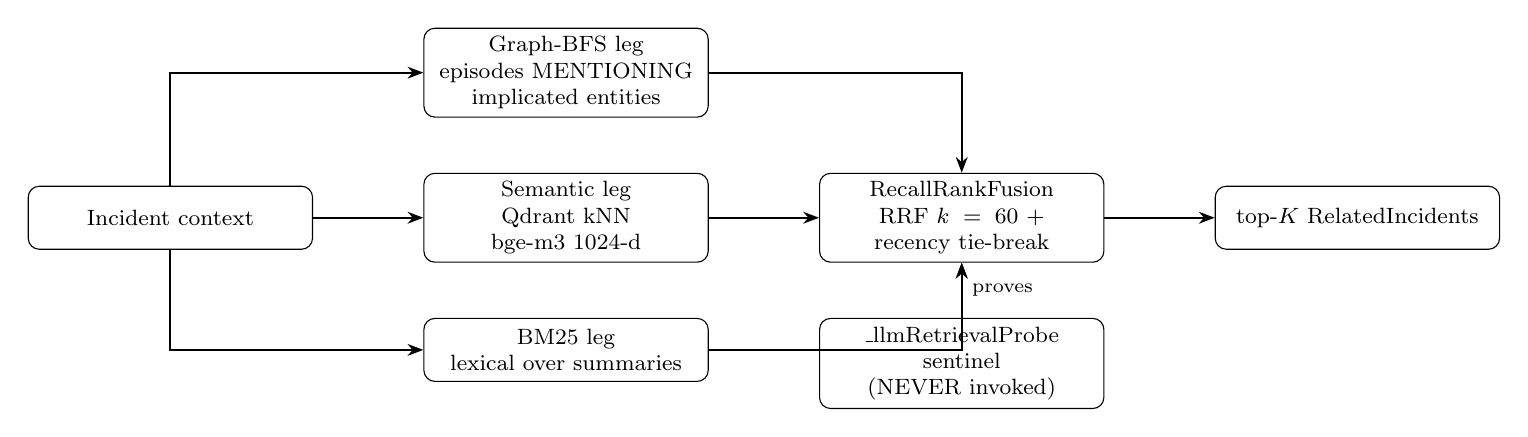
\begin{tikzpicture}[
  node distance=7mm and 14mm,
  box/.style={draw, rounded corners, align=center, font=\footnotesize,
    minimum height=8mm, inner sep=3pt, text width=34mm},
  arr/.style={-{Stealth[length=2mm]}, thick}
]
\node[box] (inc) {Incident context};
\node[box, right=of inc] (sem) {Semantic leg\\Qdrant kNN bge-m3 1024-d};
\node[box, below=of sem] (bm) {BM25 leg\\lexical over summaries};
\node[box, above=of sem] (bfs) {Graph-BFS leg\\episodes MENTIONING\\implicated entities};
\node[box, right=of sem] (rrf) {RecallRankFusion\\RRF $k=60$ + recency tie-break};
\node[box, right=of rrf] (top) {top-$K$ RelatedIncidents};
\node[box, below=of rrf, text width=34mm] (probe) {\_llmRetrievalProbe sentinel\\(NEVER invoked)};

\draw[arr] (inc) -- (sem);
\draw[arr] (inc.north) |- (bfs.west);
\draw[arr] (inc.south) |- (bm.west);
\draw[arr] (bfs.east) -| (rrf.north);
\draw[arr] (sem) -- (rrf);
\draw[arr] (bm.east) -| (rrf.south);
\draw[arr] (rrf) -- (top);
\draw[arr, dashed] (probe.north) -- (rrf.south) node[midway, right, font=\scriptsize] {proves};
\end{tikzpicture}
\caption{Three orthogonal recall legs fused by RRF with a recency tie-break. The
sentinel exists only to prove that no LLM is consulted on the retrieval path.}
\label{fig:recall}
\end{figure}

\begin{itemize}
  \item \textbf{Semantic leg}---a Qdrant $k$-nearest-neighbour search over the
    \texttt{incident-memory-bge-m3-v1} collection, embeddings from bge-m3 at 1024
    dimensions (Cosine). Finds incidents that \emph{read} similar even when
    wording differs.
  \item \textbf{BM25 leg}---classical lexical ranking over episode summaries.
    Catches exact symptom phrases and identifiers that dense vectors blur.
  \item \textbf{Graph-BFS leg}---\texttt{RecallEpisodesMentioningEntities} walks
    the bi-temporal subgraph for \texttt{MemoryEpisode}s that \texttt{MENTIONS}
    any of the entities the current investigation has implicated, restricted to
    currently-valid facts. This is the structural leg: it finds incidents that
    touched \emph{the same components}, not merely similar prose.
\end{itemize}

Each leg degrades to empty on failure---a down store contributes nothing rather
than throwing (\textbf{NFR-SG-2}, \textbf{AC-64}). The legs are then fused by
\texttt{RecallRankFusion.Fuse}, a pure, total, \textbf{no-LLM} function:

\begin{verbatim}
// RRF damping constant (Cormack et al.); larger k flattens rank contribution.
private const double RrfK = 60.0;

// each episode's score = sum over legs it appears in of 1/(k + rank)  (rank 0-based)
acc.Score += 1.0 / (RrfK + rank);
acc.LegCount += 1; // breadth -- how many legs this episode recurs in
\end{verbatim}

The ordering is deliberately layered to encode the Generative-Agents intuition
while staying deterministic (\textbf{NFR-SG-5}):

\begin{enumerate}
  \item \textbf{Leg breadth} (\texttt{LegCount})---an episode appearing in more
    legs outranks one ranking high in a single leg. RRF rewards breadth; we make
    it the primary key.
  \item \textbf{Recency} (\texttt{ConcludedAtEpoch})---the more-recently-concluded
    episode wins ties (the recency factor of the recency $\times$ importance
    $\times$ relevance triple).
  \item \textbf{RRF position score}---the finer tie-break under recency.
  \item \textbf{Stable fingerprint}---a final lexicographic tie-break so the order
    is total and reproducible.
\end{enumerate}

Critically, \textbf{no LLM is consulted on this path}. The recall constructor
accepts an \texttt{Action? llmRetrievalProbe} sentinel that the production path
\emph{never invokes}; a dedicated red-team unit test fails if it ever is. This is
not a comment-level promise---it is a structural guarantee enforced by the test
suite (\textbf{NFR-SG-16}), matching the Graphiti no-LLM-at-retrieval property.
The recall span records only counts and latency, never bodies
(\textbf{OBS-SG-9}).

\subsection{Reflexion lessons and the Voyager skill store}

On every conclusion the agent writes a \texttt{MemoryEpisode} and, alongside it, a
Reflexion-style lesson (\textbf{FR-SG-49}, \textbf{ADR-042}).
\texttt{ReflexionLessonRenderer} produces a recon-stripped, ID-citing ``Lesson:
cause \ldots\ resolution \ldots'' record---a verbal self-reflection in the sense
of \citet{shinn2023reflexion} that turns a closed incident into a durable,
reusable artifact. The accompanying skill store follows the Voyager discipline
\citep{wang2023voyager}: resolutions accrete into a growing library of
runbook-shaped entries the agent can recall and reuse, mitigating catastrophic
forgetting by construction---external memory rather than weight updates.

Both lesson text and recalled summaries pass through the same recon-strip on the
way \emph{in} (at write) and again on the way \emph{out} (at render)---defence-in-depth,
so no PHI-like token reaches the model frame even if one slipped past ingestion
(consistent with the \textbf{SEC-SG-7} PHI-egress guard introduced in
increment~7).

\subsection{The code$\leftrightarrow$graph join}

A recalled incident is far more useful if it links back to the code it implicated.
The static-code ingest lane embeds each structure-defining \texttt{:CodeUnit} and
persists the returned Qdrant point id onto \texttt{CodeUnit.embedding\_ref}
(\textbf{FR-SG-48}, \textbf{ADR-042}~D3)---a deterministic UUID derived from
\texttt{repo|path}. This makes the join bidirectional: graph$\to$code returns a
service's code-unit \texttt{embedding\_ref}s, and code$\to$graph maps a semantic
code hit's point id back to its owning \texttt{:Service}. When memory recall
surfaces a related incident, the agent can therefore pivot from ``this looks like
GT-03'' to the exact source file the prior episode changed.

\section{Implementation}
\label{sec:impl}

The subsystem is .NET~10, living in \texttt{src/DebugAgent/Rca/Memory/} (recall,
fusion, Reflexion rendering, recon-strip, the Qdrant upserter) and
\texttt{src/DebugAgent/StackGraph/Ingest/GraphIngestor.Memory.cs} (the bi-temporal
writer), governed by \textbf{FEAT-027} increment~6 (\textbf{FR-SG-46}--\textbf{FR-SG-49},
\textbf{NFR-SG-15}, \textbf{NFR-SG-16}, \textbf{SEC-SG-7}, \textbf{ADR-042},
\textbf{ADR-047}).

\paragraph{Why hand-rolled.}
The reference \texttt{graphiti-core} is Python/TypeScript. Running it would mean a
long-lived Python sidecar with its own image, memory footprint, and failure
surface---on a node already at roughly 96\% memory-request saturation, inside a
2~GiB FalkorDB cap, under a 50~EUR/month ceiling (\textbf{ADR-042}~D1).
\texttt{mem0} was likewise rejected. The pattern, by contrast, is small: a handful
of parameterised Cypher templates and a pure RRF function. Re-implementing it in
the language the rest of the agent already speaks costs less, operationally and
financially, than either dependency.

\paragraph{Stores and models.}
The store and model assignments are listed in Table~\ref{tab:stores}.

\begin{table}[ht]
\centering
\caption{Stores and models touching incident memory.}
\label{tab:stores}
\begin{tabular}{lll}
\toprule
Concern & Choice & Detail \\
\midrule
Graph store    & FalkorDB & \texttt{bluerobin\_stack} graph, Redis wire \texttt{:6379}, 2~GiB cap, Cypher via \texttt{GRAPH.QUERY} \\
Memory vectors & Qdrant   & \texttt{incident-memory-bge-m3-v1}, bge-m3 \textbf{1024-d}, Cosine, gRPC \texttt{:6334} \\
Code vectors   & Qdrant   & \texttt{code-embeddings}, separate collection for the code$\leftrightarrow$graph join \\
Embeddings     & in-cluster Ollama & OpenAI-compatible \texttt{/v1/embeddings}, never transits the Cloudflare edge (\textbf{ADR-020}) \\
LLM egress     & Cloudflare AI Gateway & irrelevant to recall---\emph{no model is called at retrieval} \\
\bottomrule
\end{tabular}
\end{table}

The embedding traffic is the budget-defining decision: by running bge-m3 locally
on Ollama, embeddings are effectively free and never cross the metered Cloudflare
edge. The only LLM spend touching memory is at \emph{write} time (narration for
the episode summary), not retrieval, keeping the whole recall path off the
20~EUR/month LLM line entirely. The recall latency target is the Graphiti figure:
$\approx$300~ms P95 (\textbf{NFR-SG-16}).

\paragraph{Rollout discipline.}
Memory ships shadow-first via an \texttt{RcaMemory.Mode} flag (\textbf{ADR-039}
lineage). In shadow mode the legs run, the metrics emit (\textbf{OBS-SG-9}, per-leg
hit counts and a hit-ratio warm-signal tagged by mode), and the fused result is
logged but \textbf{not} injected into the LLM frame. Only once the warm-signal
shows the collection is returning real hits does an operator flip the flag to
active. The eval gate (below) proves that flipping it does not regress
localization accuracy.

\section{Evaluation}
\label{sec:eval}

We evaluate the memory subsystem the same way the rest of the agent is
evaluated---and with the same explicit caveats. The harness \texttt{RcaEvalHarness}
replays a labelled ground-truth set through the real RCA path against a seeded,
isolated FalkorDB key (\texttt{bluerobin\_stack\_eval}), emitting a deterministic
AC@1 and a replay-clock MTTR proxy.

\paragraph{What the numbers are---and are not.}
The ground-truth set is \textbf{9 self-seeded incidents} spanning three fault
classes (auth/login, data/datastore, deploy/config), seeded from existing
synthetic tests and past runs---explicitly \emph{not} from ChaosMesh, and
explicitly disclaiming OpenRCA / ITBench-AA comparability. The repository's own
header calls the scorer-only arm ``the oversimplified-benchmark caveat.'' The MTTR
figures are \textbf{sub-second replay-clock proxies} measured by a stopwatch
around the in-process investigation call; they are not production MTTR. Real
MTTD/MTTA/MTTR p50/p95 are computed from live lifecycle data by a separate
endpoint, but no measured production values are committed.

The memory-specific result is a \textbf{no-regression ablation}, not an accuracy
gain (Table~\ref{tab:scorecard}).

\begin{table}[ht]
\centering
\caption{Memory ablation on the nine-incident self-seeded set. MTTR is a
sub-second replay-clock proxy, not production mean-time-to-resolution.}
\label{tab:scorecard}
\begin{tabular}{lcccp{4.4cm}}
\toprule
Arm & AC@1 & MTTR (replay s) & Incidents & Notes \\
\midrule
Scorer-only baseline & 1.00 & 0.0017 & 9 & AC@1 $= 1.0$ \emph{by construction} (labelled cause planted top-1) \\
Live-path baseline (distractors injected) & 1.00 & 0.0032 & 9 & the honest production-path arm; AC@1 $< 1.0$ is \emph{achievable} \\
Memory shadow (recall off frame) & 1.00 & --- & 9 & collapses to baseline byte-for-byte (the control) \\
Memory active (recall in frame) & 1.00 & --- & 9 & no regression; gate tolerance AC@1 drop $\le 0.02$, MTTR rise $\le 30$~s \\
\bottomrule
\end{tabular}
\end{table}

The honest reading: on this small, self-seeded benchmark, turning incident-memory
recall on does not \emph{break} localization, and the recall-fusion logic is
unit-proven (breadth-across-legs beats single-leg, recency tie-break, top-$K$
bounding, fail-open-to-empty). It does \textbf{not} demonstrate a measured
accuracy lift---the benchmark is too small and too clean to show one, and we do
not claim it. The contribution is the architecture and the discipline
(shadow-first, fail-open, no-LLM-at-retrieval, eval-gated), not a leaderboard
number.

For external calibration: the honest autonomous ceiling for LLM RCA is low---the
best agent on OpenRCA \citep{xu2025openrca} reaches $\approx$11\% exact-match, the
best frontier model on ITBench-AA \citep{aa2026itbenchaa} $\approx$47\%
precision@full-recall. An advisory, human-in-the-loop posture is the state of the
art, not a concession; memory is one ingredient (RCACopilot-style retrieval reuse,
\citealp{chen2024rcacopilot}) that the field expects to help, evaluated here only
for safety, not for lift.

\section{Limitations \& Threats to Validity}
\label{sec:limitations}

\begin{itemize}
  \item \textbf{Benchmark is oversimplified and self-seeded.} Nine labelled
    incidents, authored by us, with the labelled cause planted as a strong top-1.
    AC@1 $= 1.0$ in the scorer arm is by construction; even the distractor-injected
    live-path arm localizes all nine. These numbers say ``no regression,'' not
    ``accurate at scale,'' and there is real risk of the set being unrepresentative
    of production faults.
  \item \textbf{MTTR is a replay-clock proxy.} Sub-second stopwatch timings around
    an in-process call are not production mean-time-to-resolution and must not be
    read as such.
  \item \textbf{No measured accuracy lift from memory.} We show the subsystem is
    safe to enable (no regression) and internally correct (unit-proven fusion); we
    do not show it improves RCA on this benchmark, because the benchmark is too
    small to.
  \item \textbf{Shadow-first, not yet load-bearing in production.} At the time of
    writing, memory recall runs in shadow on the live path; the flip to active is
    operator-gated on a warm-signal, so production behaviour is observed but not
    yet acted on.
  \item \textbf{Construct validity of the no-LLM guarantee.} The sentinel proves
    no LLM is invoked on the \emph{retrieval} code path; episode \emph{summaries}
    are still LLM-narrated at write time. The guarantee is about retrieval, not the
    entire memory lifecycle.
  \item \textbf{Dependency-mismatch hazard.} The incident-memory and
    code-embedding Qdrant collections share configuration plumbing; a
    create-on-demand race could mint the memory collection at the wrong
    dimensionality unless the declarative init job wins---a latent operational risk
    we flag rather than hide.
  \item \textbf{Advisory by design.} A human always merges. This is positioned as
    matching the state of the art, but it does mean the memory subsystem's value is
    mediated entirely by whether it improves a human's decision---which this
    evaluation does not measure.
\end{itemize}

\section{Conclusion}

Giving an LLM RCA agent durable memory does not require a memory framework. By
re-implementing the Graphiti bi-temporal pattern as a labelled subgraph on an
already-deployed FalkorDB, the BlueRobin Debug Agent gains time-aware incident
memory---\texttt{MemoryEpisode} and deduplicated \texttt{MemoryEntity} facts
joined by bi-temporal \texttt{MENTIONS} / \texttt{RESOLVED\_BY} /
\texttt{SUPERSEDES} edges that invalidate intervals instead of deleting them,
supporting as-of queries---without a new service, a Python sidecar, or a budget
overrun. Retrieval is a three-leg hybrid (semantic + BM25 + graph-BFS) fused by
Reciprocal Rank Fusion with a Generative-Agents recency tie-break and a structural
sentinel proving no model is consulted, complemented by Reflexion lessons, a
Voyager-style skill store, and a code$\leftrightarrow$graph embedding join. The
honest framing is that this is an architecture-and-discipline contribution: it
ships shadow-first, it is fail-open, it consults no LLM at retrieval, and it is
gated by a deliberately oversimplified self-seeded benchmark that proves safety
rather than a leaderboard win---all at a $\approx$50~EUR/month homelab cost. That
combination---production-grade, graph-grounded, temporally-correct agent memory at
hobbyist cost---is the point.

\bibliographystyle{plainnat}
\bibliography{references}

\end{document}
